\begin{savequote}[8cm]
Alles Gescheite ist schon gedacht worden.\\
Man muss nur versuchen, es noch einmal zu denken.

All intelligent thoughts have already been thought;\\
what is necessary is only to try to think them again.
  \qauthor{--- Johann Wolfgang von Goethe \cite{von_goethe_wilhelm_1829}}

\end{savequote}

\chapter{\label{ch:nu-theo}The Theory of Neutrinos}
\minitoc
The main goal of neutrino experiments is to measure all neutrino properties, including the mass, mixing angles, and the CP violation parameter, $\dcp$. 
The mixing angles and $\dcp$ fully describes neutrino oscillation, while the mass is the reason why neutrino oscillation happens.
Hence, these parameters will be better illustrated in the following Sec.~\ref{sec:oscillation} in the context of the theoretical framework of neutrino oscillation.
As only products from neutrino interaction are detected in experiments, to achieve the said goal, a good understanding of neutrino interaction is necessary.
Hence, a brief overview of neutrino interaction is given in Sec.~\ref{sec:interaction}.

\section{Oscillation}
\label{sec:oscillation}
Neutrinos come in three flavours: electron neutrino ($\nu_e$), muon neutrino ($\nu_\mu$), and tau neutrino ($\nu_\tau$).
The different flavours of neutrinos will only produce the corresponding lepton in weak interaction, so they are eigenstates of the weak interaction.
However, neutrinos propagate through space as mass eigenstates, $\nu_1$, $\nu_2$, and $\nu_3$.
The reason for neutrino oscillation to occur is two-fold.
One is beacuse the mass eigenstates do not have a simple one-to-one correspondence with the weak eigenstates. 
They are a superposition of the weak eigenstates and vice versa.
The other is beacuse these mass eigenstates have different masses.
Neutrinos are created as flavour eigenstates in weak interaction, but they propagate as a linear combination of mass eigenstates, which propagate with different phase velocities due to their different masses.
Hence, throughout the propagation, the linear combination of mass eigenstates is changing constantly, leading to a changing superposition of flavour eigenstates, and thus, neutrino oscillation.

To be more specific, the matrix describing the mixing of mass eigenstates to flavour eigenstates is the PMNS matrix.
It is conventionally parameterized as follows:

\begin{equation}
U_{\text{PMNS}} = 
\begin{pmatrix}
1 & 0 & 0 \\
0 & c_{23} & s_{23} \\
0 & -s_{23} & c_{23}
\end{pmatrix}
\begin{pmatrix}
c_{13} & 0 & s_{13} e^{-i\dcp} \\
0 & 1 & 0 \\
-s_{13} e^{i\dcp} & 0 & c_{13}
\end{pmatrix}
\begin{pmatrix}
c_{12} & s_{12} & 0 \\
-s_{12} & c_{12} & 0 \\
0 & 0 & 1
\end{pmatrix}
\end{equation}
where $c_{ij} = \cos\theta_{ij}$ and $s_{ij} = \sin\theta_{ij}$, and $\dcp$ is the CP violation phase.
The angles, $\theta_{ij}$, are the mixing angles. 
Using the PMNS matrix, the flavour eigenstates can be expressed in terms of the mass eigenstates as follows:
\begin{equation}
\begin{pmatrix}
\nu_e \\
\nu_\mu \\
\nu_\tau
\end{pmatrix}
=
U_{\text{PMNS}}
\begin{pmatrix}
\nu_1 \\
\nu_2 \\
\nu_3
\end{pmatrix}
\end{equation}
To keep a close focus on the development of the theoretical idea, detailed derivations are rendered to the Appendix~\ref{app:oscillation}, and only important results are included here for elaboration.
Due to the small neutrino masses, the mass eigenstate, with mass $m_i$, acquires a phase approximately of
\begin{equation}
  \ket{\nu_i(L)} = e^{-i \frac{m_i^2L}{2E}} \ket{\nu_i(0)},
\end{equation}
after travelling a distance $L$ with energy $E$.
Hence, the probability of a neutrino of flavour $\alpha$ at creation to be detected as a neutrino of flavour $\beta$ after travelling a distance of $L$ is given by
\begin{array}{rl}
  P_{(\alpha \to \beta)} &= \left|\braket{\nu_\beta | \nu_\alpha(L)} \right|^2 = \left| \sum_i U_{\alpha i} U^*_{\beta i} e^{-i \frac{m_i^2L}{2E}} \right|^2 \\
  &= \delta_{\alpha\beta} - 4 \sum_{i>j} \text{Re} \left( U_{\alpha i} U^*_{\beta i} U^*_{\alpha j} U_{\beta j} \right) \sin^2 \left( \frac{\Delta m^2_{ij} L}{4E} \right) \\
  &+ 2 \sum_{i>j} \text{Im} \left( U_{\alpha i} U^*_{\beta i} U^*_{\alpha j} U_{\beta j} \right) \sin \left( \frac{\Delta m^2_{ij} L}{2E} \right),
\end{array}
where $\delta{\alpha\beta}$ is the Kronecker delta, $U_{\alpha i}$ is the element of the PMNS matrix, and $\Delta m^2_{ij} = m_i^2 - m_j^2$.
This result shows that the oscillation probability depends on the mixing angle through the PMNS matrix elements and on the mass difference and neutrino energy through the sine terms.
For brevity, the dependence on the sine terms can be characterised by a phase angle,
\begin{equation}
  \label{eq:osc-phase}
  \Delta_{ij} = \frac{\Delta m^2_{ij} L}{2E} \approx 1.27 \frac{\Delta m^2_{ij} [\text{eV}^2] L [\text{km}]}{E [\text{GeV}]},
\end{equation}
where the oscillation is maximal when $\Delta_{ij} = \pi / 2$.
These results can be used to better understand how the various parameters are measured in different types of neutrino experiments.
The different sensitivies of these experiments are due to the relatively large difference in the mixing angles and the mass differences.
The latest values for the neutrino parameters based on Ref.~\cite{Capozzi:2021fjo,ParticleDataGroup:2024cfk} are given in Table~\ref{tab:neutrino-parameters}, which shows that the magnitude of $\delta_{21}$ is much smaller than that of $\delta_{31}$.
Unlike the CKM matrix, where all mixing angles are small, only $\theta_{13}$ is small while the other two angles are considerably larger, suggesting significant mixing.

\begin{table}[h]
  \centering
  \begin{tabular}{c|c|c}
    Parameter & Value & Sensitive Experiment\\
    \hline
    \hline
    $\Delta m^2_{21}~(\ev^2)$ & $7.36^{+0.16}_{-0.15} \times 10^{-5}$ & Reactor and solar \\
    $|\Delta m^2_{31}|~(\ev^2)$ & $2.448^{+0.023}_{-0.031} \times 10^{-3}$ & Atmospheric \\
    $\theta_{12}$ ($\deg$) & $33.40^{+0.80}_{0.82}$ & Reactor and solar \\
    $\theta_{23}$ ($\deg$)       & $42.4^{+1.0}_{0.9}$ & Atmospheric\\
    $\theta_{13}$ ($\deg$)       & $8.59^{+0.13}_{0.12}$ & Reactor and solar \\
    $\dcp$ ($\deg$) & $223^{+32}_{-23}$   & Accelerator and atmospheric \\
    \hline
  \end{tabular}
  \caption{The latest values for the neutrino parameters.}
  \label{tab:neutrino-parameters}
\end{table}



\subsection{Atmospheric neutrinos}
  Atmospheric neutrinos are mostly muon neutrinos produced from decays of mesons produced by cosmic rays interacting with the atmosphere.
  The neutrino energy is typically of the order of $1~\gev$, while the distrance travelled has a range of $O(10^2)$ to $O(10^4)~\km$.
  Substituting these numbers into \Eq.~\ref{eq:osc-phase}, $\Delta_{23}$ is of the order of $O(10^{-2})$ to $O(1)$, while $\Delta_{21}$ is of the order of $O(10^{-3})$ to $O(10^{-1})$.
  Hence, oscillation is much more prominent in the $\nu_\mu \to \nu_\tau$ channel than in the $\nu_\mu \to \nu_e$ channel.
  This is why atmospheric neutrino experiments are sensitive to $\theta_{23}$ and $\Delta m^2_{32}$, which are sometimes referred to as the atmospheric mixing angle and mass difference, respectively.

\subsection{Reactor neutrinos}
  Reactor neutrinos are mostly electron antineutrinos produced from nuclear fission in the power plants.
  The neutrino energy is typically of the order of $1~\mev$.
  Unlike the atmospheric neutrino measurement, detectors can be placed at various locations to measure different parameters.
  Thus, it is easier to discuss reactor neutrino oscillation by introducing the oscillation length variable given as:
  \begin{equation}
    \label{eq:osc-length}
    L_{\text{osc}} = \frac{4\pi E}{\Delta m^2} = 2.48 \frac{E [\text{MeV}]}{\Delta m^2 [\text{eV}^2]} \text{m},
  \end{equation}
  which corresponds to one complete period of neutrino oscillation.
  Substituting the reactor neutrino energy into Eq.~\ref{eq:osc-length}, one gets $L_{\text{osc}} = O(10^2)~\km$ for $\delmtwoo$ and $L_{\text{osc}} = O(1)~\km$ for $\delmthro$. 
  Hence, by placing detectors kilometers away from the power plants, reactor neutrino experiments offer the unique opportunity to measure $\tothr$ and $\delmthro$, which are sometimes referred to as the reactor mixing angle and mass difference, respectively.
  Additionally, placing detectors at around $O(100)~\km$ away from the power plants allows the measurement of $\delmtwoo$.

  \subsubsection{Solar neutrinos}
  Solar neutrinos are mostly electron neutrinos produced from nuclear fusion in the sun.
  The majority of solar neutrinos have energies below $1~\mev$, except those from the $^8$B decay, which have energies up to $15~\mev$.
  The distance travelled by solar neutrinos is of the order of $O(10^8)~\km$.
  Substituting these values into Eq.~\ref{eq:osc-length}, one gets $L_{\text{osc}} = O(10^4)~\m$ for $\delmtwoo$ and $L_{\text{osc}} = O(10^3)~\m$ for $\delmthro$.
  Both are much smaller than the average distance travelled, so to observe the clear oscillatory pattern like in other neutrino experiments, the exact distance travelled by the individual neutrino needs to be known with an incredibly high precision, which is beyond the current detection capability.
  Fortunately, the average oscillation result can still be measured by the total survival rate of the electron neutrinos.
  
  On top of the usual neutrino oscillation, there is another important phenonemon at play in the solar neutrino measurements, which is the Mihheev-Smirnov-Wolfenstein (MSW) effect~\cite{Wolfenstein:1977ue,Mikheyev:1985zog}.
  A full discussion on the MSW effect is beyond the scope of this thesis.
  Simply put, the MSW effect is the modification of the mixing parameters due to the presence of electrons in matter. 
  This modification can enhance or suppress the oscillation probability depending on the mass difference and the electron density.
  Approximately, the required electron density is proportional to the mass difference squared and inversely proportional to the neutrino energy.
  Hence, the lower the neutrino energy or the larger the mass difference, the higher the electron density is required to modify the oscillation probability.
  Due to the considerably larger $\delmthro$, for almost the whole energy range of solar neutrinos, the electron density in the Sun is not sufficient to modify the mixing between $\nu_1$ and $\nu_3$.
  As for the relatively smaller $\delmtwoo$, the electron density is high enough to significantly modify the mixing between $\nu_1$ and $\nu_2$ for the high energy neutrinos from the $^8$B decay.
  The resultant impact on these high energy electron neutrinos is an alteration of its composition of the mass eigenstates such that when they leave the surface of the Sun, they are mainly composed of $\nu_2$, a considerably larger fraction than the unmodified composition.
  The MSW effect is demonstrated when different experiments measure solar neutrinos with different energies and observe a different survival rate of electron neutrinos.
  The absolute survival rates are sensitive to $\totwo$ and $\tothr$ for the low energy region and the high energy region, respectively.


\subsection{Accelerator neutrinos}
  In accelerator neutrino experiments, there is relatively greater freedom than in other types of neutrino experiments as both the neutrino source and the detector are designed to optimize osicllation.
  This section uses T2K as an example, but the underlying principles are common to all LBL experiments.
  More details of the T2K experiment will be illustrated in Chapter~\ref{ch:t2k}.

  Neutrinos are produced in accelerators by bombarding protons on some form of target, carbon in the case of T2K, to produce an abundance of mesons.
  The charged mesons can be redirected to point in the desired direction using sophisticated magnetic horn.
  Besides directionality, the magnetic horn can also select the mesons of the desired charge.
  For example, positive (negative) pions can be focused if a beam of muon (anti-)neutrinos are needed.
  It is this control over the neutrino source that enables accelerator experiments to measure $\dcp$.
  As the neutrino energy from the meson decay is angular dependent, it is possible to obtain a beam of neutrinos with different energy spread by varying the angle of the detector respective to the beam direction. 
  T2K places its detectors at $2.5\deg$ off-axis to obtain a neutrino beam narrow in energy distribution with a peak at $0.6~\gev$.
  According to Eq.~\ref{eq:osc-phase}, to achieve maximal oscillation, the far detector needs to be placed at a length of approximately $300$~km from the source for the larger mass difference, i.e. $\delmthrt\approx\delmthro\approx2.5\times10^{-3}~\eV$.
  This is why accelerator measurments are sensitive to $\tttthr$.
  By analysing oscillation in the neutrino mode and in the anti-neutrino mode, T2K is able to extract the best-fit value of $\dcp$ that could describe the collected data~\cite{T2K:2019bcf}.
  However, the current measurement is heavily limited by statistics and thus has large uncertainties.
  In the Hyper-K era, the statistics is expected to increase significantly, and to maximize the potential of the measurement, a commensurate reduction in systematic uncertainties is of paramount importance.
  This leads us naturally to the discussion of one of the major systemtics in neutrino experiments, neutrino interactions.

\section{Interaction}
\label{sec:interaction}
The underlying theory for neutrino oscillation is straightforward, and the parameters to be measured are clear, but the experimental determination of these parameters is challenging.
Due to the weak interaction of neutrinos, they cannot be detected directly.
All neutrino measurements are based on the detection of the particles produced in the neutrino interaction.
Therefore, to extract the desired neutrino oscillation parameters with a high precision, a good understanding of neutrino interactions is crucial.
This chapter provides the basic understanding of neutrino interactions necessary for the interpretation of the analyses presented in the subsequent chapters.

\subsection{$\nu$-quark}
The most fundamental interaction between a neutrino and matter is the weak interactions between the neutrino and a quark, the Feynman diagrams for which are shown in Fig.~\ref{fig:nu-q-feyn}.

\begin{figure}[h]
  \centering
  \begin{subfigure}[b]{0.45\textwidth}
    \centering
    \begin{tikzpicture}
      \begin{feynman}
        \vertex (a) {\(\nu_\ell\)};
        \vertex [right=of a] (b);
        \vertex [right=of b] (c) {\(\ell\)};
        \vertex [below=of b] (d);
        \vertex [left=of d] (e) {\(q\)};
        \vertex [right=of d] (f) {\(q'\)};
        
        \diagram* {
          (a) -- [fermion] (b) -- [fermion] (c),
          (b) -- [boson, edge label=\(W\)] (d),
          (e) -- [fermion] (d) -- [fermion] (f),
        };
      \end{feynman}
    \end{tikzpicture}
    \caption{Charge current interaction.}
    \label{fig:cc-interaction}
  \end{subfigure}
  \hfill
  \begin{subfigure}[b]{0.45\textwidth}
    \centering
    \begin{tikzpicture}
      \begin{feynman}
        \vertex (a) {\(\nu_\ell\)};
        \vertex [right=of a] (b);
        \vertex [right=of b] (c) {\(\nu_\ell\)};
        \vertex [below=of b] (d);
        \vertex [left=of d] (e) {\(q\)};
        \vertex [right=of d] (f) {\(q\)};
        
        \diagram* {
          (a) -- [fermion] (b) -- [fermion] (c),
          (b) -- [boson, edge label=\(Z\)] (d),
          (e) -- [fermion] (d) -- [fermion] (f),
        };
      \end{feynman}
    \end{tikzpicture}
    \caption{Neutral current interaction.}
    \label{fig:nc-interaction}
  \end{subfigure}
  \caption{Feynman diagrams for neutrino interactions with a quark.}
  \label{fig:nu-q-feyn}
\end{figure}
More specifically, Fig.~\ref{fig:cc-interaction} is mediated by the $W$ boson and the neutrino is converted to a charged lepton, while Fig.~\ref{fig:nc-interaction} is mediated by the $Z$ boson and the neutrino remains a neutrino.
The former is the charged current (CC) interaction, while the latter is the neutral current (NC) interaction.
Following the Feynman diagram, it is straightforward to write down the amplitude for the interaction.
The amplitude for the CC interaction is given by:
\begin{equation}
  \mathcal{M}_{\text{CC}} = \frac{g^2}{2} \bar{u}_\ell(p') \gamma^\mu (1 - \gamma^5) u_\nu(p) \frac{-i g_{\mu\nu}}{q^2 - M_W^2} \bar{u}_q(k') \gamma^\nu (1 - \gamma^5) u_q(k),
\end{equation}
where $g$ is the weak coupling constant, $u_\ell$ and $u_\nu$ are the spinors for the outgoing lepton and incoming neutrino, respectively, $u_q$ are the spinors for the quarks, $q$ is the momentum transfer, and $M_W$ is the mass of the $W$ boson.
This interaction takes place only when the neutrino possesses high enough energy <how high?> to probe inside the nucleon and interact with the quarks.
The product quark will hadronize and produce a jet of particles.
This type of interaction is refered to as deep inelastic scattering (DIS).
DIS is highly complicated, but no so relevant for this thesis, so will not be discussed further.
More details can be found in reviews, such as Ref.~\cite{}. <DIS review>

\subsection{$\nu$-nucleon}
  At the T2K beam energy, the predominant fraction of the neutrinos do not possess the energy to probe inside the nucleon, but rather interact with the nucleon as a whole.
  Depending on the specific neutrino energy, the interaction can be classified as quasi-elastic (QE), resonance, or deep inelastic scattering (DIS).

    \subsubsection{QE}
    Although at the quark level, the interaction appears to the same as the $\nu$-quark interaction shown in Fig.~\ref{fig:nu-q-feyn}, the interacted quark cannot be treated as independent, but rather as part of a nucleon.
    Hence, the effective $\nu$-nucleon interaction feynman diagram is shown in Fig.~\ref{fig:nu-n-feyn}.
    \begin{figure}[h]
      \centering
      \begin{subfigure}[b]{0.45\textwidth}
        \centering
        \begin{tikzpicture}
          \begin{feynman}
            \vertex (a) {\(\nu_\ell\)};
            \vertex [right=of a] (b);
            \vertex [right=of b] (c) {\(\ell\)};
            \vertex [below=of b] (d);
            \vertex [left=of d] (e) {\(N\)};
            \vertex [right=of d] (f) {\(N'\)};
            
            \diagram* {
              (a) -- [fermion] (b) -- [fermion] (c),
              (b) -- [boson, edge label=\(W\)] (d),
              (e) -- [fermion] (d) -- [fermion] (f),
            };
          \end{feynman}
        \end{tikzpicture}
        \caption{Charge current interaction.}
        \label{fig:cc-interaction-n}
      \end{subfigure}
      \hfill
      \begin{subfigure}[b]{0.45\textwidth}
        \centering
        \begin{tikzpicture}
          \begin{feynman}
            \vertex (a) {\(\nu_\ell\)};
            \vertex [right=of a] (b);
            \vertex [right=of b] (c) {\(\nu_\ell\)};
            \vertex [below=of b] (d);
            \vertex [left=of d] (e) {\(N\)};
            \vertex [right=of d] (f) {\(N\)};
            
            \diagram* {
              (a) -- [fermion] (b) -- [fermion] (c),
              (b) -- [boson, edge label=\(Z\)] (d),
              (e) -- [fermion] (d) -- [fermion] (f),
            };
          \end{feynman}
        \end{tikzpicture}
        \caption{Neutral current interaction.}
        \label{fig:nc-interaction-n}
      \end{subfigure}
      \caption{Feynman diagrams for neutrino interactions with a nucleon.}
      \label{fig:nu-n-feyn}
    \end{figure}
    The leptonic current remains the same, but the hadronic current is now a nucleon current instead of a quark current.
    Hence, the hadronic current is much more complicated and and comprises of several form factors, which paramterize our understanding of the nucleon structure.
    For instance, the hadronic current for the CC interaction is given by:
    \begin{array}
      \mathcal{M}_{\text{CC}} = \frac{G_F}{\sqrt{2}} \bar{u}_\ell(p') \gamma^\mu (1 - \gamma^5) u_\nu(p) \\
       \bar{u}_N(k') \left[ F_1(q^2) \gamma_\mu + F_2(q^2) \frac{i \sigma_{\mu\nu} q^\nu}{2M} + F_A(q^2) \gamma_\mu \gamma^5 + F_P(q^2) \frac{q_\mu \gamma^5}{m_\pi} \right] u_N(k),
    \end{array}
    where $G_F$ is the Fermi constant, $F_1$, $F_2$, $F_A$, and $F_P$ are the form factors, $M$ is the nucleon mass, and $m_\pi$ is the pion mass.
    The derivation is complicated and beyond the scope of this thesis. 
    More details can be found in Ref.~\cite{LlewellynSmith:1978te}.
    It is however important to note that $F_1$ and $F_2$ are the vector form factors, which can be extracted from the electron scattering measurements, and $F_P$ is the pseudoscalar form factor, which can be related to $F_A$, the axial form factor, through the Partially Conserved Axial Current Hypothesis (PCAC) .
    Hence, the axial form factor is unique to neutrion experiments and can only be extracted from past measurements.
    Fig.~\ref{fig:cc0pi} shows an event display of a candidate $\cczpi$ event, which is likely a QE event, in the upgraded ND280 during the beam run in Jun. 2024.
    \begin{figure}[!htb] 	
        \centering 		
        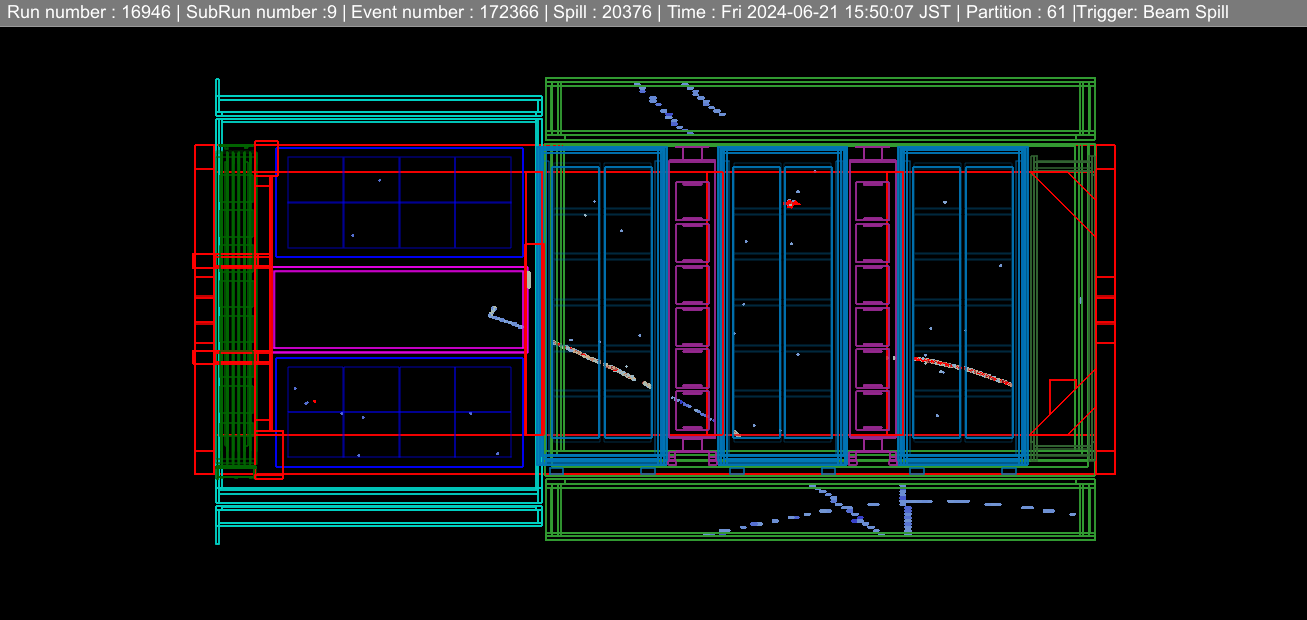
\includegraphics[width=\sgfigwid\textwidth]{figures/cc0pi.png}
        \caption{\label{fig:cc0pi} A $\cczpi$ candidate event in upgraded ND280, where the long track is the primary muon and the short track is the primary proton.} 
    \end{figure}

    \subsubsection{Resonance}
    When the neutrino energy is high enough to excite the nucleon to a higher energy state, e.g. $\Delta(1232)$ the interaction is classified as a resonance interaction.
    The excited nucleon then decays to produce a pion. 
    Hence, the resonance modelling is sometimes used interchangeably with the single pion production modelling.
    One of the most common moodel used today is the Berger-Sehgal model, which improves from the earlier Rein-Sehgal model by taking into account the effect of the lepton mass. (CHECK)
    The Rein-Sehgal model is based on the approximate relativistic quark model in Ref.~\cite{Feynman:1971wr}.
    Subsequent developments such as the MK model~\cite{Kabirnezhad:2017jmf,Kabirnezhad:2020wtp,Kabirnezhad:2022znc}, provides more sophisticated calculations.

    Fig.~\ref{fig:cc1pi} shows an event display of a candidate $\ccopi$ event, which is likely a resonance event, in the upgraded ND280 during the beam run in Jun. 2024.
    \begin{figure}[!htb] 	
        \centering 		
        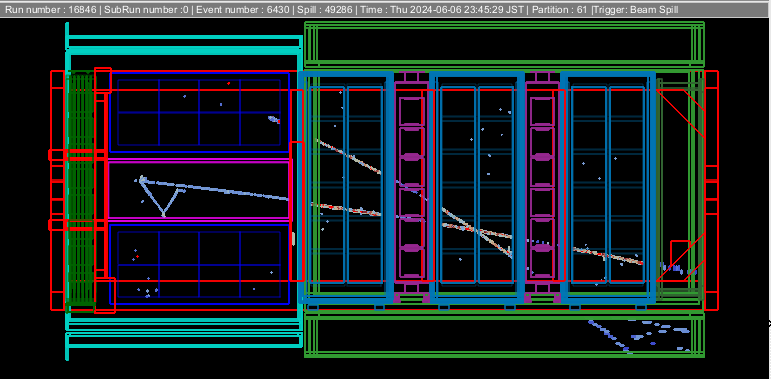
\includegraphics[width=\sgfigwid\textwidth]{figures/shortME.png}
        \caption{\label{fig:cc1pi} A $\ccopi$ candidate event in upgraded ND280, where the long track is the primary muon and the V-shaped track is identified as a pion track by the short delayed track, identified as the Michel electron, attached to its end.} 
      \end{figure}
  
  \subsection{$\nu$-nucleus}
  Modern day neutrino experiments employ heavier elements, such as hydrocarbon and argon, to increase event rates.
  This further complicates the neutrino interaction.
  The simplest case is for the relatively high energy neutrino, for which the Impulse Approximation (IA) can be used.
  The neutrino sees the nucleon as independent from other nucleons, so the interaction approaches the $\nu$-N interaction.
  Even in this simplest case, the presence of the nuclear medium still affects the interaction in two ways, namely the intial state (IS) effect and the final state interaction (FSI).

  When the neutrino energy drops, IA is no longer valid and can only resolve the nucleus as a whole.
  In this case, Random Phase Approximation (RPA) correction is needed, which is beyond the scope of this thesis and will not be ellaborated further. 
  Interest readers can refer to REFXXX for more details.
  Instead, the two nuclear effects will be elaborated further below.

    \subsubsection{Initial state}
    The nuclear effects manifest in two ways.
    Firstly, the nucleon in the interaction is in a bound state, i.e. it cannot have arbitrary energy and momentum like a free nucleon.
    Instead, the energy distribution of the nucleon is parameterised by the so-called Spectral Function (SF).
    The simplest form of SF is the Fermi Gas model, which treats the nucleons as freely moving Fermi gas.
    Hence, the nucleon momentum is filled up to the Fermi momentum, which is given as:
    <CHECK>
    \begin{equation}
        k_F = (3\pi^2 \rho/2)^{1/3},
    \end{equation}
    where $\rho$ is the nuclear density.
    <How is the fermi momentum determined?>
    This model oversimplifies the nuclear structure.
    A more realistic model is the local Fermi gas (LFG) model, which accounts for the varying nuclear density, leading to an SF of the form:
    (CHECK)
    \begin{equation}
        S(k, E) = \int \rho(\vec{r}) \delta(E - \sqrt{k^2 + m^2}) d^3r,
    \end{equation}
    where $m$ is the nucleon mass.

    Further improvement, such as the short-range correlation between nucleons that increases the high momentum fraction.
    There are also effective SFs. Fit to data?

    \subsubsection{FSI}
    \label{sec:nuint-fsi}
    The second nuclear effect is the Final State Interaction (FSI).
    Regardless of how the neutrino interacts with the nucleon, the interaction products are still inside the nucleus.
    They have to propagate through the nuclear medium to be detectable.
    The interactions with the nuclear medium are classified as FSI.
    They are more pronounced for hadrons than leptons, as the former are more likely to interact with the nuclear medium.
    There are several types of FSI, such as the elastic scattering, charge exchange, and absorption.
    \begin{enumerate}
        \item 
    CEX involves changing the charge of the participating particles; for example,
    \begin{equation}
        \pip + \n \rightarrow \piz + \p,
    \end{equation}
    or vice versa. This rescattering type is crucial for event topologies requiring the presence of a pion;  depending on the signal pion charge, CEX could migrate events between signal and background. 
  
    \item 
    INEL is the case where the nucleus is left in an excited state after the rescattering. This category only contains the situation where a single additional nucleon is emitted/knocked-out after rescattering. Since it does not affect the number of pions produced, it will not convert an event from a pionless topology to a pion-production topology. The effects on nucleons are two-fold. Firstly, it can alter the number of signal events within each event topology. If the inelastic rescattering leads to two low-momentum protons below the detection threshold as opposed to a high-momentum proton, this signal event will be discarded as no protons are observed. Secondly, INEL invariably changes the kinematics of the rescattering particle. Be it the leading proton or the leading pion, based on which the TKI observables are calculated, the TKI distribution shape will be affected. Hence, while $\ninel$ would affect all four data sets, $\piinel$ would only affect \ttkpip and \minpiz. 
  
    \item 
    ABS refers to the case where the particle undergoes an interaction so that it does not emerge as a final particle. For example, $\pi^+$ can interact with two or more nucleons, initially forming a baryon resonance that subsequently interacts with other nucleons, emitting multiple nucleons rather than pions. Hence, the $\pi^+$ would not emerge from the nucleus anymore.
  
    \item 
    PIPD happens for energetic particles where an extra pion emerges as a result of the rescattering, such as
    \begin{equation}
        \p + \p \rightarrow \p + \n + \pip.
    \end{equation}
    Such an interaction significantly alters the event topology. 
  
    \end{enumerate}
  
  
  

    \subsubsection{TKI}
    \label{sec:nuint-tki}
    Due to the heavy target nucleus in present neutrino experiments, nuclear effects are almost inextricable for conventional single particle kinematic measurement.
    This highly impeds model development, as nuclear effects can micmic different $\nu$-N processes.
    For instance, if the proton produced from a QE $\nu$-N interaction has high enough energy to produce an additional pion during FSI, which propagates out of the nucleus.
    This QE event will micmic the output of a resonance interaction, or in term of topology, this CC$0\pi$ event will micmic a CC$1\pi$ event.
    Hence, nuclear effects such as pion production can alter cross section measurements of different topologies differently, thereby impacting the modelling of the main underlying $\nu$-N interaction processes.
    Therefore, an accurate description of the nuclear effect is crucial for reducing model systematics.
    To gain insights on nuclear effects, observables that are particularly sensitive to these effects are indispensable. 
    The Transverse Kinematic Imbalance (TKI) varaibles are exactly one such set of observables~\cite{Lu:2015hea, Lu:2015tcr}.
    The TKI variables are shown in Fig.~\ref{fig:stki}.
    \begin{figure}[!htb] 	
        \centering 		
        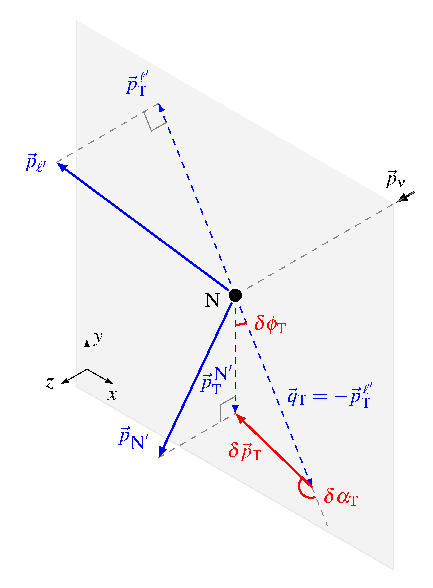
\includegraphics[width=0.35\textwidth]{figures/stki.eps}
        \caption{\label{fig:stki} Schematic illustration of the TKI variables. Diagram taken from Ref.~\cite{Lu:2015tcr}.} 
    \end{figure}
    In the simplest case, there are only two final particles after the neutrino-nucleon interaction, a muon and a proton. 
    In the absence of nuclear effects, the muon and the proton should be emitted with momenta of the same magnitude but opposite direction in the plane transverse to the neutrino direction.
    The TKI variables are constructed to quantify the deviation from this ideal scenario in measurements to access the nuclear effects. 
    The presence of IS will affect the initial nucleon momentum, so the sum of the muon and proton transverse momenta will deviate from zero, which is quantified by $\dpt$, and their direction will not be exactly opposite, which is quantified by $\dphit$.
    Furthermore, if the nucleus is assumed to be at rest and no other particles are knocked out other than the muon and the proton, the initial nucleon momentum, $\pn$, can also be estimated following the steps outlined in Ref.~\cite{Furmanski:2016wqo, Lu:2019nmf}. 
    This esimation amounts to an approxiate  $\mathcal{O}(20\%)$ correction~\cite{Yang:2023dxk}. 
    Hence, $\dpt$ and $\pn$ serve as good probes for IS models.
    FSI will smear these distributions, but the shape and the peak position is mostly due to IS modelling.
    All current IS models do not have a preferential direction for initial nuclear motion, so it is natural to assume the nucleons move in random directions isotropically, leading to a uniform $\dat$ distribution, which is the angle between the initial nucleon momentum and the proton momentum in the tranvserse plane. 
    Thus, the deviation from flatness for $\dat$ can only be due to FSI, thereby making it an excellent probe for FSI. 
    
    In the case of pion production, an additional doouble transverse variable, $\dptt$, can be constructed by projecting $\vecdpt$ onto the direction perpendicular to the lepton scattering plane, which is defined as the plane containing $\vecpl$ and $\vecpnu$.
    The reconstruction is illustrated in Fig.~\ref{fig:dtki}.
    \begin{figure}
        \centering
        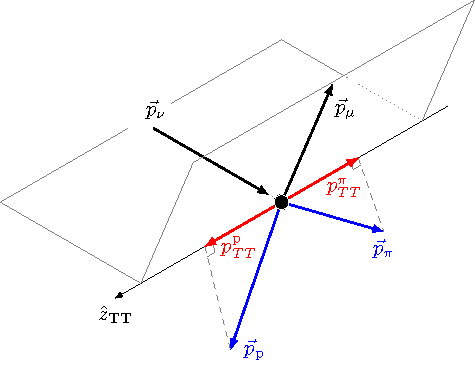
\includegraphics[width=0.35\textwidth]{figures/dptt.pdf}
        \caption{\label{fig:dtki} Schematic illustration of the double TKI variable, $\dptt$. Diagram taken from Ref.~\cite{T2K:2021naz}.}
    \end{figure}
    In the absence of nuclear effects, $\dptt$ should be zero.
    The spread of the $\dptt$ distribution is sensitive to the nuclear effects in pion production~\cite{MINERvA:2020anu, T2K:2021naz}.
    Its equivalent in pionless production, $\dptx$, has been proposed and studied together with its orthogonal companion, $\dpty$, in MINERvA~\cite{MINERvA:2019ope}.
    Additionally, Ref.~\ref{Lu:2015tcr,Hamacher-Baumann:2020ogq} suggests the possibility of using $\dptt$ to select a $\nu$-H sample.
    Further details on a hydrogen sample selection will be discussed in Sec.~\ref{sec:mc-hyrdrogen}.
    
    There has been a wealth of measurements from various neutrino experiments such as  T2K~\cite{T2K:2018rnz, T2K:2021naz}, MINERvA~\cite{MINERvA:2018hba, MINERvA:2019ope, MINERvA:2020anu, MINERvA:2021csy}, and MicroBooNE~\cite{MicroBooNE:2022emb, MicroBooNE:2023cmw, MicroBooNE:2023tzj, MicroBooNE:2023wzy, MicroBooNE:2024tmp}.
    As the TKI idea is equally applicable to electron scattering, experiments such as CLAS~\cite{CLAS:2021neh} has also produced TKI measurments, showcasing the efficacy and wide applicability of TKI. 


% This document introduction won't serve as a complete primer on \LaTeX.  There are plenty of those online, and googling your questions will often get you answers, especially from \url{http://tex.stackexchange.com}.

% Instead, let's talk a little about a few of the features and packages lumped into this template situation.  The \verb|savequote| environment at the beginning of chapters can add some wittiness to your thesis.  If you don't like the quotes, just remove that block.

% For when it comes time to do corrections, there are two useful commands here.  First, the \verb|mccorrect| command allows you to highlight a short correction \mccorrect{like this one}.  When the thesis is typeset normally, the correction will just appear as part of the text.  However, when you declare \verb|\correctionstrue| in the main \verb|Oxford_Thesis.tex| file, that correction will be highlighted in blue.  That might be useful for submitting a post-viva, corrected copy to your examiners so they can quickly verify you've completed the task.

% \begin{mccorrection}
% For larger chunks, like this paragraph or indeed entire figures, you can use the \verb|mccorrection| environment.  This environment highlights paragraph-sized and larger blocks with the same blue colour.
% \end{mccorrection}
